\section{Downsampling}
\subsection{Simple and Complex Downsampling}
An image can be easily downsampled by a factor of $N$ by only considering every $N$\textsuperscript{th} pixel. In MATLAB this can be done by indexing the image array using a range, \lstinline|I(1:N:end, 1:N:end)|. However, this naïve implementation has a few problems. Since downsampling has the effect of compacting the images of the baseband signal in the frequency domain, a phenomenon known as aliasing occurs. This happens when the images of the signal overlap with the baseband signal. The moire patterns that can be seen in the middle image in Figure \ref{fig:DownsampledImages}. \\
The proper way to downsample an image is to first apply a lowpass filter to the image. In the frequency domain, this removes the high frequency information thereby creating a larger separation between the baseband signal and its images. This then lowers the chance of aliasing when we downsample the image. The improvement over the naïve downsampling approach is evident when looking at the last image in Figure \ref{fig:DownsampledImages}.
\begin{figure}[H]
    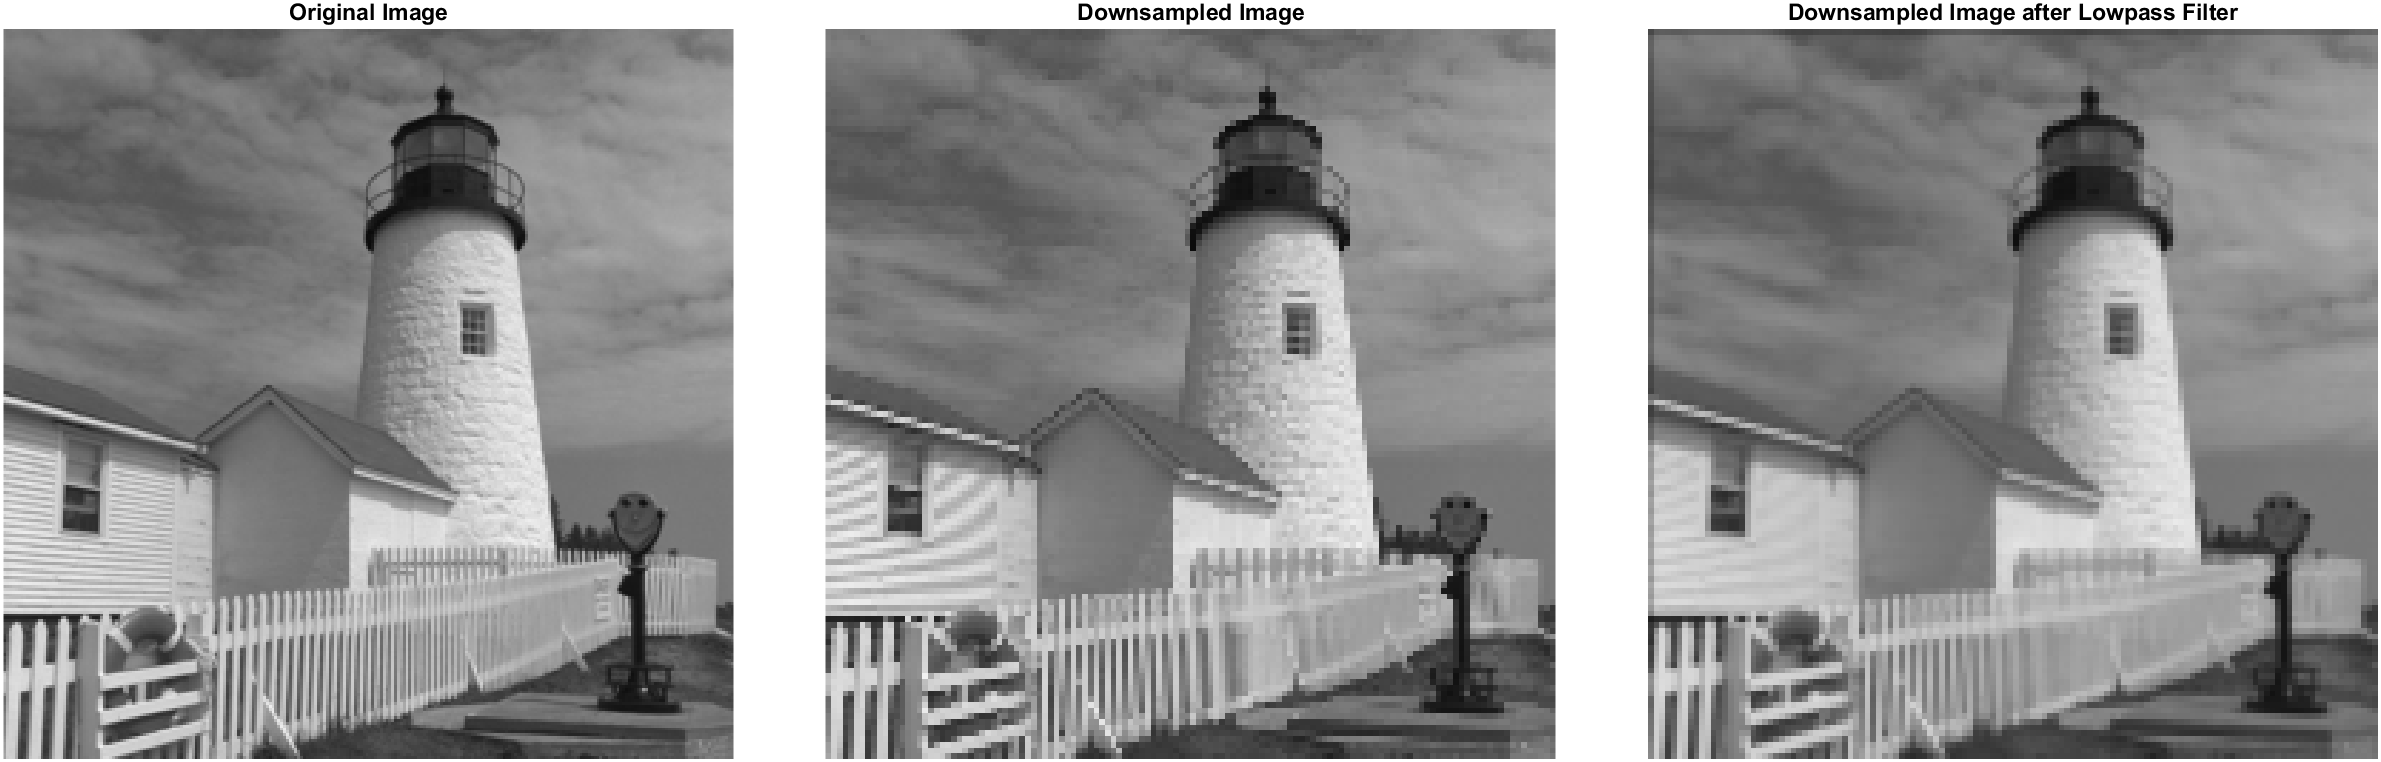
\includegraphics[width=1\textwidth]{DownsampledImages.png}
    \centering
    \caption{Original and Downsampled Images}
    \label{fig:DownsampledImages}
\end{figure}